\chapter{问题分析和研究框架}
\label{cha:problem_framework}

\section{本章引论}

随着互联网上不同类型的平台出现,人们每天在各种平台上产生着各种各样的行为和发言。如现在微博平台上会对热门时事设置井号标签,人们透过加上对应标签来表达对该事件的想法,以及透过对这些发言进行赞点、分享或评论来表达支持或反驳。利用井号标签收集数据并进行意图分析可以得知网民对该事件的舆论方向。在其他平台上的各种行为记录同样可能有挖掘其意图的价值,意图识别的应用场景也变得多种多样,但即使数据的内容和结构不同,问题的本质是相似的。

本章的内容安排如下。在章节\ref{sec:global_problem_analysis}中,我们将首先针对意图识别进行分析,并给出统一的形式化表示。基于该形式化表示,在章节\ref{sec:global_framework}中,我们再进一步提出一个面向社交媒体文本的意图识别研究框架。从原始文本的输入到最终识别目标的输出,理清其中每个步骤的功能和目的,给出一个完整识别系统的设计方案,为解决后续章节中研究的问题准备一个统一的切入点。

\section{问题分析}
\label{sec:global_problem_analysis}

本小节中,我们将对意图识别中涉及的各个元素作出分析,并给出统一的形式化表示来描述他们的相互关系。

不同意图识别问题中都有要被识别的意图倾向$C$。如Tang等人\cite{tang2015learning}的情感极性识别研究,$C$对应需要五级的情感极性。在刘丹丹等人\cite{刘丹丹2015基于}的微博情感分类研究中,$C$对应喜好、安乐、惊奇、厌恶、悲哀、愤恨、恐惧。邓钊等人\cite{2015面向微博的中文反语识别研究}的中文反语识别研究中,$C$则对应是否包含反讽。

其次是研究主体$T$,它是行为发起者$S$的行为记录,可以认为他表达想法和情感的载体。另外一些场景下会有背景信息$B$,对应所有有助于正确理解$T$的信息。譬如要研究讨论区上帖子的意图倾向,那么$T$就是帖子的内容,包括其中的文本内容、图片、文件附件等,$S$则是帖子的发布者。而帖子所在讨论区的类型有助于定位帖子对应的领域,发布者的发布历史显示发布者的一些态度倾向,帖子下的评论从侧表反映主帖的内容,这些就是背景信息$B$,都可能是理解帖子内容的提示。又以Zahiri等人\cite{Zahiri2017Emotion}对电视剧台词的情感识别研究为例,那么$T$指电视剧中的台词,$S$则是发出这段台词的对应角色,$B$则是台词的上文,其中包含其他角色正在谈论的内容,这些角色和发言者的关系是什么,说话的氛围如何等等,都能对台词的内容有更明确的定位。

意图识别假设对于任意一个研究样本$t \in T$,在给定背景信息$b \in B$(或某些情况下假设与背景信息无关),其承载想法或情感必然存在对应的倾向$c \in C$。意图识别首先要从样本主体和背景信息中分别提取出与识别目标相关的信息$f_t$和$f_b$,即需要提出两个映射函数,$F_T$和$F_B$,满足 $f_t=F_T(t)$和$f_b=F_B(b)$。再进一步根据相关信息识别出其想法或情感倾向,即找出一个映射关系$F_C$,使得 $c=F_C(f_t, f_b)=F_C(F_T(t), F_B(b))$。

\begin{figure}[H]
  \centering
  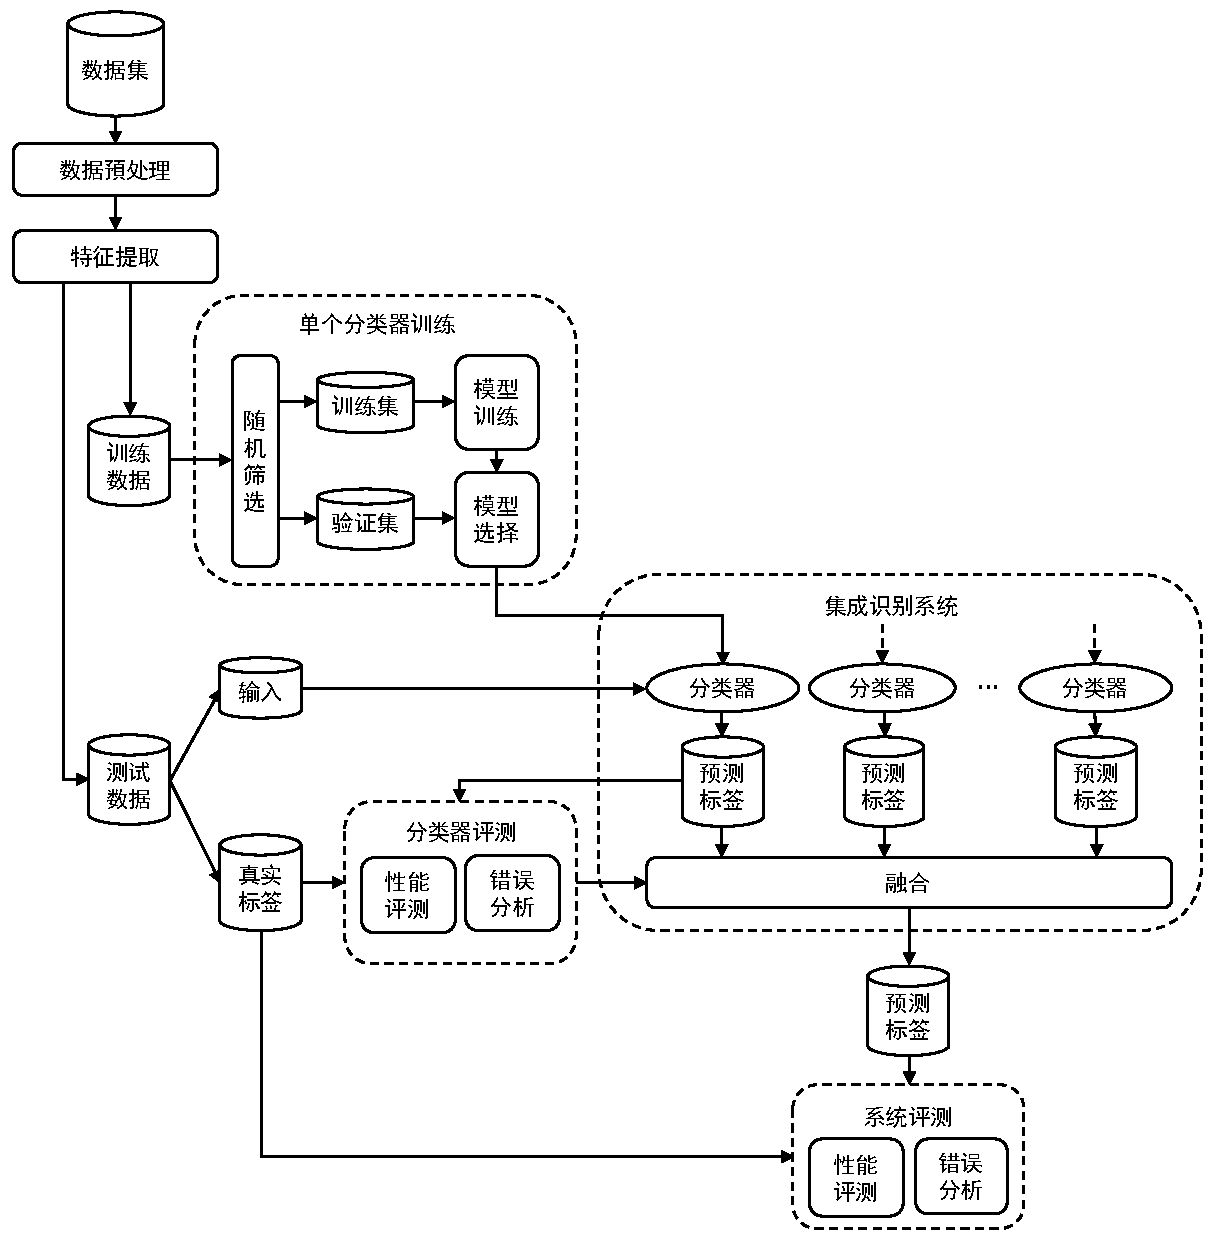
\includegraphics[width=\textwidth]{img/framework.pdf}
  \caption{意图识别的研究框架}
  \label{fig:framework}
\end{figure}

\section{研究框架}
\label{sec:global_framework}

在本小节,我们将根据前述的形式化表示给出一个意图识别的研究框架。由于在本论文的后续研究均面向英语社交媒体文本的分类问题,我们会针对此研究方法对框架进行细化,从原始文本的输入到最终识别目标的输出,理清其中每个步骤的功能和目的,给出一个集成系统的设计框架。针对不同的应用的场景,在后续实验章节中将给出具体的实现方案。

\subsection{框架入口}

图~\ref{fig:framework}显示本文面向意图识别的研究框架。整个框架的输入是实验的数据集,数据集的每个样本包含三个元素,分别是研究的主体、背景信息和意图的倾向。参考前一小节的形式化表示,一个样本可以表示为 $<t, b, c> \in T \times B \times C$。不论是训练数据或测试数据,他们都采用相同的数据预处理技术和特征提取技术来获取样本的特征,以用作分类器的输入,即透过$F_T$和$F_B$分别获取$f_t=F_T(t)$和$f_b=F_B(b)$。

\subsection{基础分类器}

在特征提取完成后,识别模型的输入就准备好了。接下来首先对基础分类器进行研究和分析,比较不同模型和不同参数在对应问题上的整体性能。对于机器学习方法,在模型的训练过程中,需要将训练数据会分成训练集和验证集两个部分。训练集用于调整模型的参数,根据预先设计的损失函数计算模型当前的预测结果和实际标签的偏差,透过微分计算出参数的调整方向,并以一定的学习步长逐步迭代。由于以上训练过程在数学逻辑上是以达到训练集上的最优解来调整参数,会出现对训练样本过拟合的问题,因此会采用验证集来评估模型对训练集以外的样本的识别性能。在每一轮参数调整后计算当前模型在验证集上的性能指标,最后选择其中最优的一轮参数作为该次模型训练最终的参数。

除了分析不同模型在对应问题上的整体性能,透过对被分类器错误识别的样本进行观察,我们需要分析单个分类器的性能局限在哪,分类器对哪些类别的样本有更高的正确率或召回率,哪些样本之间容易出现混淆,或者在输入数据当中是否存在一些有关键信息的特征没有被成功提取。特别地意图识别的研究课题中,我们会关注数据集标签的正确性。在实验的过程中我们假设标签是正确,但有研究指出自动标注会引入噪声\cite{littlestone1988learning},人工标注则难以避免地存在主观性。虽然对不同算法之间的性能比较影响不大,但对于技术水平的评估有其分析的价值。

\subsection{集成识别系统}

经过对基础分类器的分析后,我们对不同模型的识别性能有了深入的了解。为了进一步达到更好的性能,
下一步是基于基础分类器研究集成识别系统的策略和设计。我们提出了一种集成系统的设计方案,结合多个模型相同的分类器的预测结果来作出最终判断,旨在只使用一种模型的基础上尽可能提升识别的性能,或针对特定的性能指标对整个系统的识别倾向进行调整。参考决策树,其识别过程可以认为是一系列的决策,每一步决策都建立在前一步的决策结果上,并且只关注原始问题中的子问题。类似地,我们提出的集成系统经过多次决策来对样本进行意图识别,第一步先由一个分类器或多个分类器的预测结果融合得到一个基础的预测结果,接下来的每一步需要先对前一步的混淆矩阵进行分析,根据哪些类别的样本被误判对指标的影响较大,设定一个子识别任务,从训练数据中筛选出相关的子集来训练新的基础分类器,得出针对该子识别任务的决策结果,决定是否修改上一步中的预测结果。这一方法的原理在于相同的模型在相同配置下的拟合能力是有限的,而子识别任务是原始问题的简化,模型可以专注于拟合一个局部问题,并对前一步的预测结果提出修改意见,起着补丁的作用。具体方法将在后续实验章节中给出详细说明。

同样地,我们需要分析集成系统的性能。在测试数据上,观察系统经过每一轮决策调整之后的识别性能变化,验证系统框架的设计是否满足假设。另外深入观察混淆矩阵的变化,分析各个子识别任务有效的原因,判断其适用和不适用的场景。

\section{本章小结}

在本章我们首先对意图识别给出统一的形式化表示,引出了其中涉及的各个元素并描述他们的相互关系。然后描述了我们面向意图识别的研究框架,其中包括了两个研究重点。一是研究以不同算法得到的分类器对研究问题的整体性能,并作深入的分析,包括单个算法对不同类别样本的识别能力、比较不同算法在不同指标上的区别以理解他们的拟合倾向、观察被错误识别的样本并找出其原因等。二是研究基于基础分类器的集成系统,鉴于单个分类器的识别能力有限,我们提出了一个集成系统的设计方案,旨在结合多个基础分类器的预测结果来得出最终的判断,从而充分发挥一个数学模型的拟合能力,细节实现方法将在后续具体的应用场景中给出说明。



